% preambolo per doppia compilazione HTML/PDF
\ifx\pdfoutput\undefined      % compilazione htlatex
\documentclass{article}
\DeclareGraphicsExtensions{.png, .gif, .jpg}
\newcommand{\href}[2]{\Link[#1]{}{} #2 \EndLink}
\newcommand{\hypertarget}[2]{\Link[]{}{#1} #2 \EndLink}
\newcommand{\hyperlink}[2]{\Link[]{#1}{} #2 \EndLink}
\else                         % compilazione pdflatex
\documentclass{article}
\usepackage{graphicx}
\usepackage{listings}
\usepackage{fancyhdr}
\usepackage{wrapfig}
\usepackage{multirow}
\usepackage{lscape}
\usepackage{amssymb,amsmath}
\pdfpagewidth 8.5in
\pdfpageheight 11in
\setlength\textwidth{5.7in}
\setlength\textheight{8.1in}
\setlength\oddsidemargin{0in}
\setlength\evensidemargin{0in}
\setlength\topmargin{-0.6in}
\setlength\footskip{0.6in}
\setlength\headsep{0.6in}
\usepackage[hyperindex]{hyperref}
\newcommand{\percent}{\,^0\!/_0}
 \hypersetup{
    bookmarks=true,         % show bookmarks bar?
    unicode=false,          % non-Latin characters in Acrobat’s bookmarks
    pdftoolbar=true,        % show Acrobat’s toolbar?
    pdfmenubar=true,        % show Acrobat’s menu?
    pdffitwindow=true,      % page fit to window when opened
    pdfauthor={Maurizio},   % author
    pdfsubject={Ungaro},    % subject of the document
    pdfnewwindow=true,      % links in new window
    colorlinks=true,        % false: boxed links; true: colored links
    linkcolor=black,        % color of internal links
    citecolor=blue,         % color of links to bibliography
    filecolor=magenta,      % color of file links
    urlcolor=blue           % color of external links
}
\fi


\begin{document}
\pagestyle{fancy}
\renewcommand{\sectionmark}[1]{\markright{\slshape \thesection\ #1}{}}
\fancyhead[R]{\bf\rightmark} 
\fancyhead[L]{e1-6 analysis}
\fancyfoot[R]{ \sl M. Ungaro, K. Joo}
\fancyfoot[L]{ \sl UCONN/JLAB}

\title{\large e1-6 Vertex Correction, Selection}
 \author{M. Ungaro, K. Joo}
\maketitle

\abstract{This document describes the track vertex correction and selection procedure.
The track vertices of all particles are corrected. A selection on the electron and proton
z-vertexes and their differences is applied.}

\tableofcontents

\section{Vertex Correction, Selection}

In the reconstruction software the track vertex $(x,y,z)$ is calculated
from its intersection with the sector midplane\footnote{The midplane of
a sector is defined by the plane that divide that sector in half and contains
the beamline $(0,0,z)$.} of the corresponding sector. This procedure involve
the assumption that the beam is centered along the z-axis. During the e1-6 
experiment however the beam was not centered at $(x,y) = (0,0)$ thus 
a sector-dependent offset  is introduced in the vertex calculation. 


\subsection{Beam Offset}
The displacement of the beam can be seen in Fig.~\ref{fig:vertex_id}, where the events
on the window\footnote{A window was placed at $z=+0.5$ cm to help these kind of 
studies and to be a z-position reference.} downstream of the target were 
selected to fix the z position as reference. The calculated displacement
\cite{bib:valeri_vertex} for the beam position is:
$$
\begin{array}{c c c}
 x_0 = & 0.090   & cm \\
 y_0 = & -0.345 & cm
\end{array}
$$

\begin{figure}[ht]
	\centering
		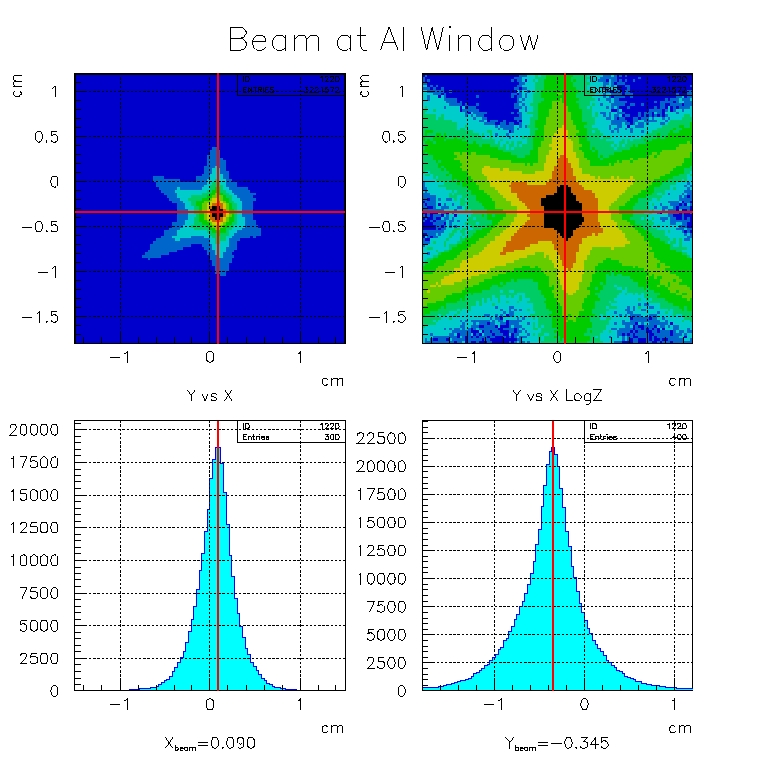
\includegraphics[width=0.65\textwidth ]{img/beam_displacement.jpg}
			\caption{Top: y versus x position of the vertex at the window.
						Upper right: same as upper left, except plotted logarithmically.
	               One can see that the beam spot was slightly shifted from $(0,0)$.
						Bottom: the x (left) and y (right) distributions which led to
						the calculation: $(x_0, y_0) = (0.09, -0.345)cm$ }
			\label{fig:vertex_id}
\end{figure}

\clearpage\newpage

\subsection{Vertex Correction, Cut}
To correct the vertex position it is sufficient to shift the midplanes
so that they contain the correct beamline $(0.09, -0.345, z)$ and recalculate 
the intersection of the tracks with the new planes.
This is illustrated in Fig.\ref{fig:vertex}.

\begin{figure}[h]
	\centering
		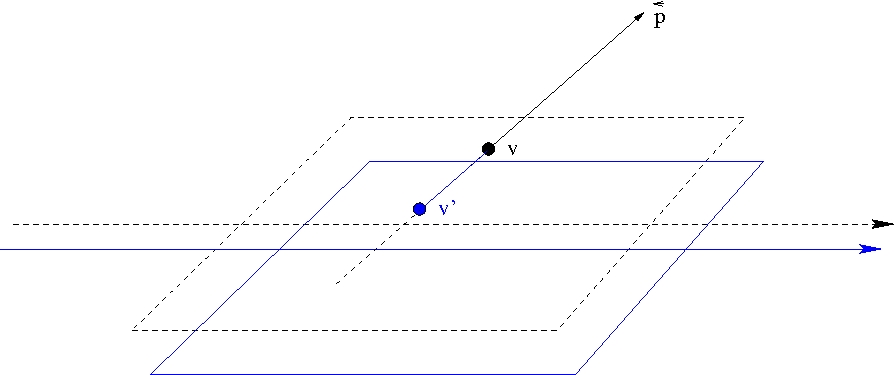
\includegraphics[width=0.98\textwidth ]{img/corr_vertex.jpg}
			\caption{The vertex correction. The dashed plane is the original midplane
						containing the wrong beamline $(0, 0, 0)$. The point $v$ is the 
						intersection of the track (straight line along momentum $\vec p$)
						with this plane. The solid blue plane represents the corrected
						midplane containing $(0.09, -0.345, z)$. The correction algorithm 
						simply intersects the same track with the corrected midplane. }
			\label{fig:vertex}
\end{figure}


\vspace{1cm}
The effect of the correction on the electrons and protons z position
is shown in Fig. \ref{fig:vertex_corr}. 
After this correction, the vertex position resolution is good enough to
introduce a cut on the z vertex of electron and protons in order to
select events inside the target cell as follows:
\begin{equation}
 -8\, cm \le z \le -0.8\, cm
\label{eqn:vertex_cut1} 
\end{equation}

The electron and proton vertices are also required to be coincident along the $z$ axis
within the reconstruction resolution, so an additional cut on
$\Delta z = z_{electron} - z_{proton}$ is applied:

\begin{equation}
 \left| \Delta z \right| < 3 \,cm
 \label{eqn:vertex_cut2} 
\end{equation}

The effect of the corrections and the values of the cuts are illustrated in 
Fig. \ref{fig:vertex_corr} and  Fig. \ref{fig:vertex_corr_2D}.

\begin{figure}[h]
	\centering
		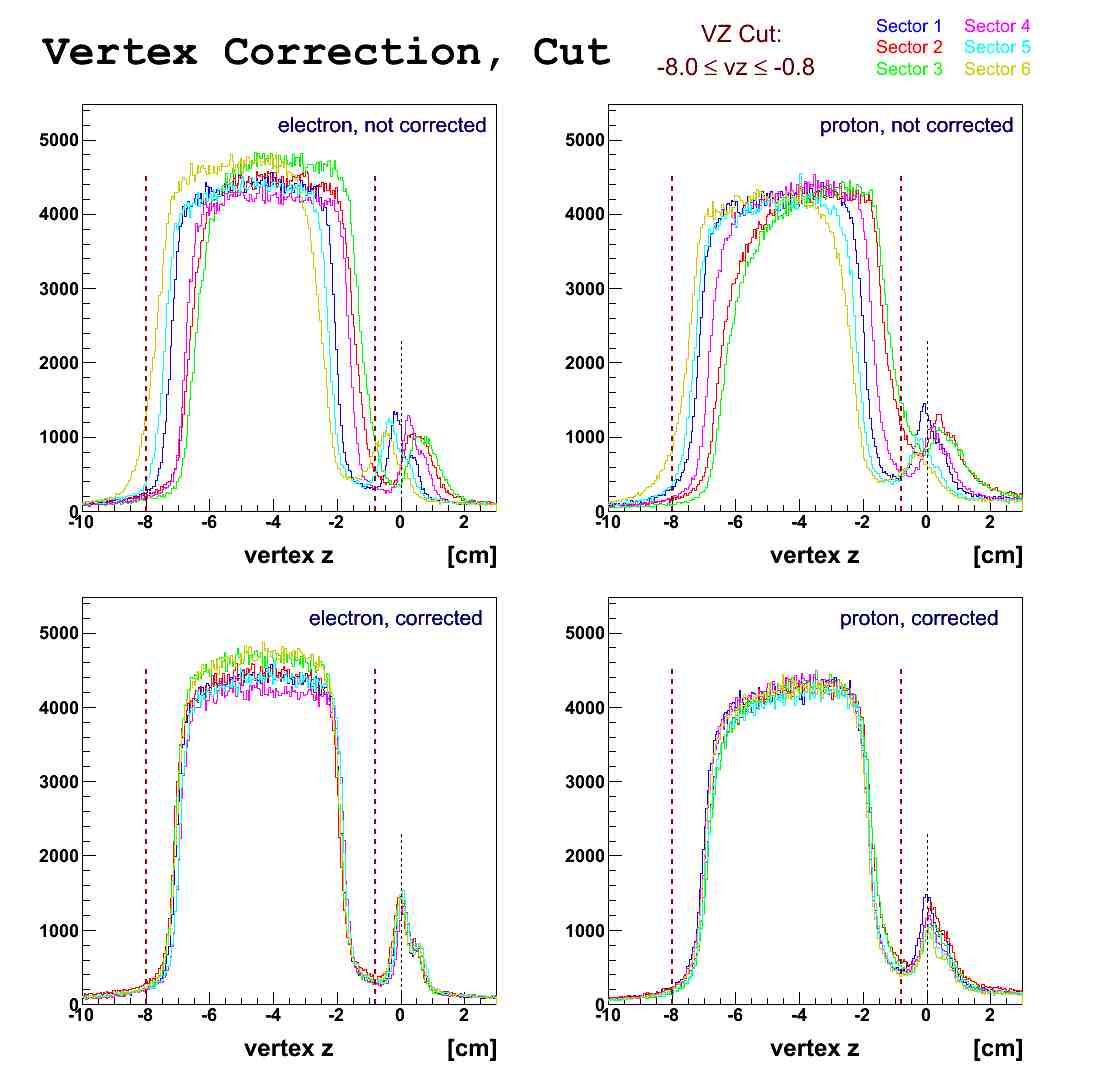
\includegraphics[width=0.96\textwidth ]{img/vtx_all_sector.jpg}
			\caption{The effect of the correction on the electrons and protons z 
						distributions for each sector. Top row: electron and proton
						z vertices, uncorrected. Bottom row: same distributions after
						the vertex correction. Vertical red lines: cuts of eq.\ref{eqn:vertex_cut1}. }
			\label{fig:vertex_corr}
\end{figure}

\begin{figure}[h]
	\centering
		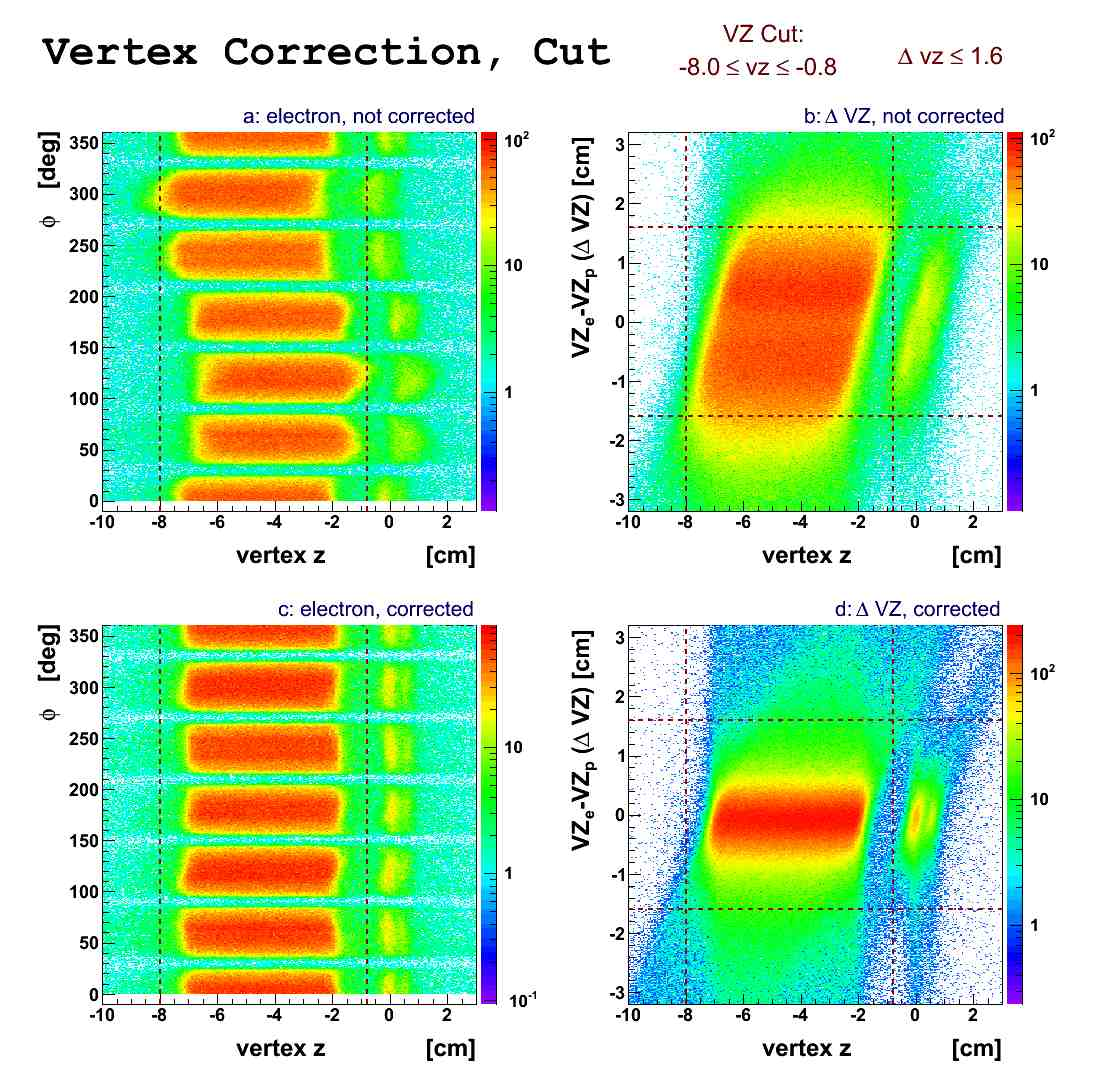
\includegraphics[width=0.96\textwidth ]{img/vtx_2D_all_sector.jpg}
			\caption{Top left: $\Delta z$ versus $\phi_{electron}$, uncorrected.
						The typical sinusodial behaviour as a function of sector is
						indicative of the beam displacement. Bottom left: same 
						distributions, after the vertex correction. 
						Top right:  $\Delta z$ versus $VZ_{electron}$, uncorrected. Bottom
						right: same distributions, after the vertex correction.
						Vertical red lines: cuts of eq.\ref{eqn:vertex_cut1}.
						Horizontal red lines: cuts of eq.\ref{eqn:vertex_cut2}.}
			\label{fig:vertex_corr_2D}
\end{figure}











\begin{thebibliography}{mybib}
 \bibitem {bib:valeri_vertex}   {Valeri Koubarovski},     {\it Private Communication.}
\end{thebibliography}


\end{document}








